\subsection*{Teil C: Geometrie (25 Minuten)}
\textit{(Wiederholung aus Arbeitsblatt 3)}

\begin{enumerate}[label=\arabic*., resume]

    \item \textbf{Symmetrie erkennen:}

    \vspace{0.5cm}

    \begin{center}
        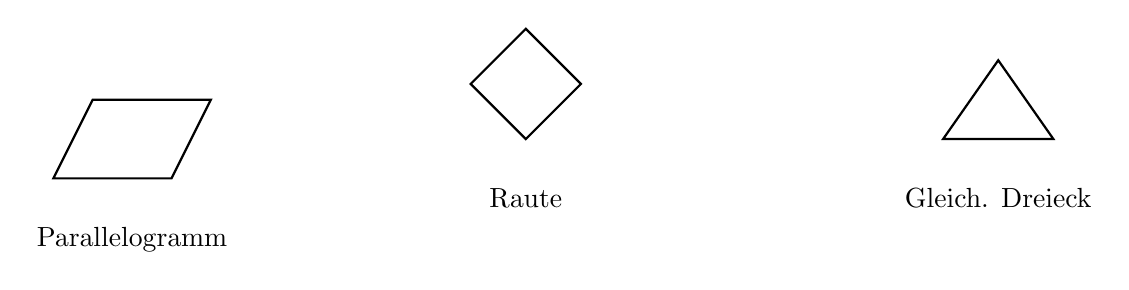
\begin{tikzpicture}[scale=1]
            % Parallelogramm
            \begin{scope}[xshift=-6cm]
                \draw[thick] (0,0) -- (1.5,0) -- (2,1) -- (0.5,1) -- cycle;
                \node[below] at (1,-0.5) {Parallelogramm};
            \end{scope}

            % Raute
            \begin{scope}[xshift=0cm]
                \draw[thick] (0,0.5) -- (0.7,1.2) -- (0,1.9) -- (-0.7,1.2) -- cycle;
                \node[below] at (0,0) {Raute};
            \end{scope}

            % Gleichseitiges Dreieck
            \begin{scope}[xshift=6cm]
                \draw[thick] (0,1.5) -- (-0.7,0.5) -- (0.7,0.5) -- cycle;
                \node[below] at (0,0) {Gleich. Dreieck};
            \end{scope}
        \end{tikzpicture}
    \end{center}

    Kreuze an:
    \begin{center}
        \begin{tabular}{|l|c|c|c|}
            \hline
            Figur & achsensymmetrisch & punktsymmetrisch & beide \\
            \hline
            Parallelogramm & $\square$ & $\square$ & $\square$ \\
            \hline
            Raute & $\square$ & $\square$ & $\square$ \\
            \hline
            Gleichseitiges Dreieck & $\square$ & $\square$ & $\square$ \\
            \hline
        \end{tabular}
    \end{center}

    \vspace{1cm}

    \item \textbf{Winkelberechnung:}

    \vspace{0.5cm}

    \begin{center}
        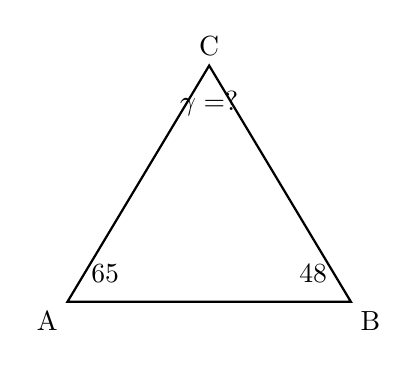
\begin{tikzpicture}[scale=1.2]
            % Dreieck
            \draw[thick] (0,0) -- (3,0) -- (1.5,2.5) -- cycle;

            % Winkel markieren
            \node at (0.4,0.3) {$65°$};
            \node at (2.6,0.3) {$48°$};
            \node at (1.5,2.1) {$\gamma = ?$};

            % Punkte beschriften
            \node[below left] at (0,0) {A};
            \node[below right] at (3,0) {B};
            \node[above] at (1.5,2.5) {C};
        \end{tikzpicture}
    \end{center}

    Berechne den Winkel $\gamma$:

    $\gamma = 180° - 65° - 48° = $ \underline{\hspace{3cm}}

    \vspace{1cm}

    \item \textbf{Winkel an parallelen Geraden:}

    \vspace{0.5cm}

    \begin{center}
        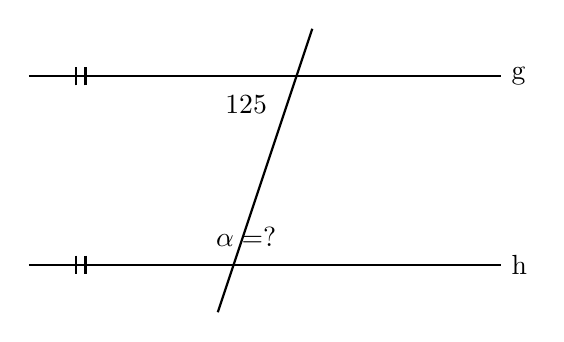
\begin{tikzpicture}[scale=1.2]
            % Parallele Geraden
            \draw[thick] (-2,1) -- (3,1) node[right] {g};
            \draw[thick] (-2,-1) -- (3,-1) node[right] {h};
            \draw[thick] (0,-1.5) -- (1,1.5);

            % Winkel markieren  
            \node at (0.3,0.7) {$125°$};
            \node at (0.3,-0.7) {$\alpha = ?$};

            % Parallele Zeichen
            \foreach \x in {-1.5,-1.4}
            {
                \draw[thick] (\x,0.9) -- (\x,1.1);
                \draw[thick] (\x,-0.9) -- (\x,-1.1);
            }
        \end{tikzpicture}
    \end{center}

    Die Geraden g und h sind parallel.

    $\alpha = $ \underline{\hspace{2cm}} (Begründung: \underline{\hspace{4cm}})

    \vspace{1cm}

    \item \textbf{Konstruktionsaufgabe:}

    Konstruiere die Winkelhalbierende des gegebenen Winkels (mit Zirkel und Lineal):

    \vspace{0.5cm}

    \begin{center}
        \begin{tikzpicture}[scale=1.5]
            \draw[thick] (0,0) -- (3,0);
            \draw[thick] (0,0) -- (2,2);
            \node at (0.5,0.2) {$\alpha$};
        \end{tikzpicture}
    \end{center}

    \textit{Beschreibe kurz dein Vorgehen:}

    1. \underline{\hspace{8cm}}

    2. \underline{\hspace{8cm}}

\end{enumerate}